\documentclass[a4paper,12pt]{report}
\usepackage[spanish,mexico]{babel}
\usepackage[utf8]{inputenc}
\usepackage[T1]{fontenc}
\usepackage{amsmath}
\usepackage{amssymb}
\usepackage{wasysym}
\usepackage[dvipsnames,pdftex]{color}
\usepackage[x11names]{xcolor}
\usepackage{tikz, tkz-euclide}
\usepackage[american]{circuitikz}
\usepackage{siunitx}
\usetikzlibrary{arrows}
\usepackage[colorinlistoftodos]{todonotes}
%\usepackage[left=2cm,right=1.5cm,top=1cm,bottom=1cm]{geometry}
%\usepackage{helvet}
%\renewcommand{\familydefault}{\sfdefault}
\setlength{\oddsidemargin}{0in}
\usepackage{geometry}
\geometry{a4paper, total = {180mm,270mm},
			left = 25mm, top = 20mm,
            right=15mm,bottom=20mm,%
            footskip=10mm}
\usepackage{float} 
% \setlength{\topmargin}{0in}
% \setlength{\voffset}{-0.5in}
% \setlength{\hoffset}{0.3in}
% \setlength{\textheight}{700pt}
% \setlength{\textwidth}{440pt}
% \setlength{\topskip}{0in}
% \setlength{\parskip}{2ex}
 \renewcommand{\baselinestretch}{1.5}
\usepackage{diagbox}
\usepackage{array}
\usepackage{listings}
\usepackage{caption}
%%% comandos definidos por el usuario
\begin{document}
\setcounter{page}{1}
\pagenumbering{roman}
\thispagestyle{empty}
\begin{center}
{\huge UNIVERSIDAD NACIONAL DE INGENIERÍA}\\[0.9cm]
{\Large FACULTAD DE INGENIERÍA MECÁNICA}\\[0.6in]
\end{center}
\begin{figure}[h]
\begin{center}

\includegraphics[scale=0.33]{logoUNI.png}
\vspace{0cm}
\end{center}
\end{figure}
\vspace{0.5cm}
\begin{center}
INFORME DE LABORATORIO\\
LABORATORIO DE CIRCUITOS ELÉCTRICOS\\[5mm]
{\large TEOREMAS DE THEVENIN, NORTON Y MÁXIMA POTENCIA DE TRANSFERENCIA}\\[10mm]
\vfill
LIMA - PERÚ \hfill SEPTIEMBRE 2019
\end{center}
\newpage
\thispagestyle{empty}
\begin{center}
{\Huge TEOREMAS DE THEVENIN, NORTON Y MÁXIMA POTENCIA DE TRANSFERENCIA}\\[0.7cm]
\small ENTREGADO:\\[0.05cm]
\small 25 SEPTIEMBRE 2019\\[1.2cm]
\end{center}
\begin{flushleft}
{\large ALUMNO:}\\[2cm]
\end{flushleft}
%\begin{center}
%\begin{tabular}{c@{\hspace{0.5in}}c}
%\rule[1pt]{3.14in}{1pt}\\
%Sotelo Cavero Sergio, 20172125K% & Nombre 5, 2017 \\[1.5cm]
%\end{tabular}
%\end{center}
%\begin{center}
%\begin{tabular}{c@{\hspace{0.6in}}c}
%\rule[1pt]{3.14in}{1pt}\\
%Huaroto Villavicencio Josué, 20174070I \\[2cm]
%\rule[1pt]{3.14in}{1pt}\\
%Landeo Sosa Bruno, 20174070I \\[2cm]
%\rule[1pt]{3.14in}{1pt}\\
%Quesquén Vitor Angel, 20172125K \\[2cm]
%\rule[1pt]{3.14in}{1pt}\\
%Sotelo Cavero Sergio, 20172125K \\[2cm]
%\end{tabular}
%\end{center}
\begin{center}
\begin{tabular}{c}
\rule[1pt]{3.14in}{1pt}\\
Huaroto Villavicencio Josué, 20174070I \\[2.5cm]
\end{tabular}
\end{center}

%\rule[1pt]{3.14in}{1pt}\\
%Maguiña Amaya Wladimir, 20172019F \\[3cm]
%\rule[1pt]{3.14in}{1pt}\\
%Luis Sosa Jose, 19774147I \\[3cm]
%\rule[1pt]{3.14in}{1pt}\\
%Sotelo Cavero Sergio, 20172125K
%\end{tabular}
%\end{center}
%\\[0.7cm]
{\large PROFESOR:} \\[2cm]
\begin{center}
\begin{tabular}{c}
\rule[3pt]{4.8in}{1pt}\\[1pt]
ING. SINCHI YUPANQUI, FRANCISCO 
\end{tabular}
\end{center}
\vfill
%\newpage
%\begin{center}
%{\Large \bf{RESUMEN}}
%\end{center}
\newpage
\tableofcontents
%\listoffigures
%\addcontentsline{toc}{chapter}{Índice de figuras}
\newpage
\pagenumbering{arabic} %%% esto es para regresar el modo de numeración a numeración arábiga
\setcounter{page}{1}  %%% empezamos en página 1
%\part{Introducción}
\chapter{Objetivos}
\begin{enumerate}
\item Tomar en consideración las medidas de seguridad indicadas para la realización de un buen trabajo en el laboratorio.
\item Conocer el funcionamiento del osciloscopio.
\item Conocer el funcionamiento de los diodos.
\item Aprender el proceso de rectificación de una onda.
\item Conocer mejor nuestro laboratorio de circuitos y sus alcances mediante esta experiencia.
\end{enumerate}
\chapter{Osciloscopio}
Un osciloscopio es un instrumento de visualización electrónico para la representación gráfica de señales eléctricas que pueden variar en el tiempo. Es muy usado en electrónica de señal, frecuentemente junto a un analizador de espectro. Presenta los valores de las señales eléctricas en forma de coordenadas en una pantalla, en la que normalmente el eje $X$ (horizontal) representa tiempos y el eje $Y$ (vertical) representa tensiones. La imagen así obtenida se denomina oscilograma. Suelen incluir otra entrada, llamada ``eje THRASHER'' o ``Cilindro de Wehnelt'' que controla la luminosidad del haz, permitiendo resaltar o apagar algunos segmentos de la traza.\\
Los osciloscopios, clasificados según su funcionamiento interno, pueden ser tanto analógicos como digitales, siendo el resultado mostrado idéntico en cualquiera de los dos casos.
\section{Osciloscopio digital}
En la actualidad los osciloscopios analógicos están siendo desplazados en gran medida por los osciloscopios digitales, entre otras razones por la facilidad de poder transferir las medidas a una computadora personal o pantalla LCD. En el osciloscopio digital la señal es previamente digitalizada por un conversor analógico digital. Al depender la fiabilidad de la visualización de la calidad de este componente, esta debe ser cuidada al máximo.\\
Las características y procedimientos señalados para los osciloscopios analógicos son aplicables a los digitales. Sin embargo, en estos se tienen posibilidades adicionales, tales como el disparo anticipado (pre-triggering) para la visualización de eventos de corta duración, o la memorización del oscilograma transfiriendo los datos a un PC. Esto permite comparar medidas realizadas en el mismo punto de un circuito o elemento. Existen asimismo equipos que combinan etapas analógicas y digitales.\\
La principal característica de un osciloscopio digital es la velocidad de muestreo, la misma determinara el ancho de banda máximo que puede medir el instrumento basándose en el Teorema de Nyquist. Viene expresada en MS/s (millones de samples /muestras/ por segundo).\\
La mayoría de los osciloscopios digitales en la actualidad están basados en control por FPGA (del inglés Field Programmable Gate Array), el cual es el elemento controlador del conversor analógico a digital de alta velocidad del aparato y demás circuitería interna, como memoria, buffers, entre otros.\\
Estos osciloscopios añaden prestaciones y facilidades al usuario imposibles de obtener con circuitería analógica, como los siguientes:
\begin{itemize}
\item Medida automática de valores de pico, máximos y mínimos de señal. Verdadero valor eficaz.
\item Medida de flancos de la señal y otros intervalos.
\item Captura de transitorios.
\item Cálculos avanzados, como la FFT para calcular el espectro de la señal. También sirve para medir señales de tensión.
\item Dentro del osciloscopio digital existen dos tipos que se diferencian claramente:
\end{itemize}
\begin{figure}[H]
\centering
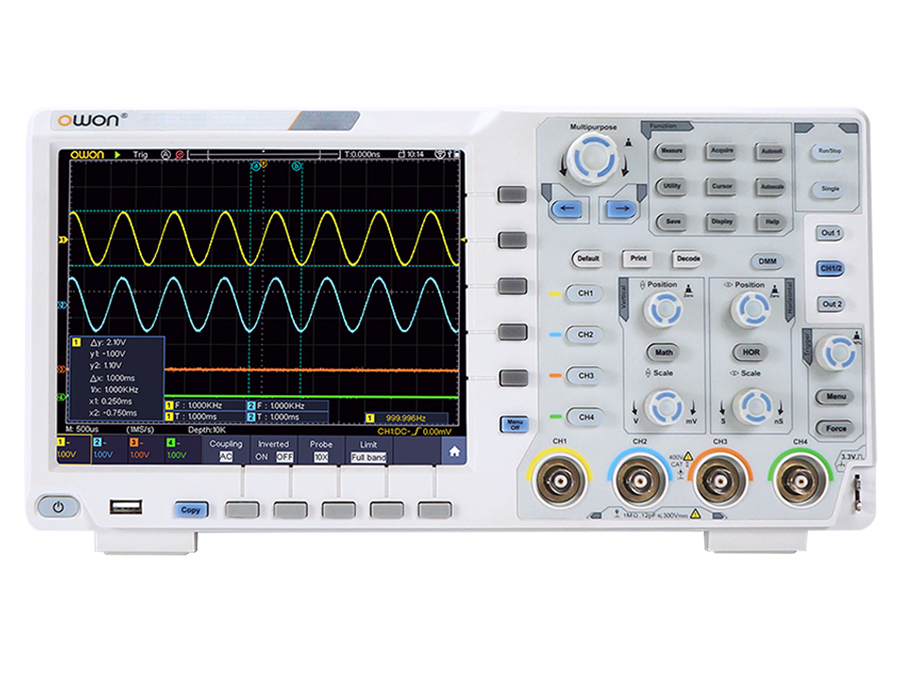
\includegraphics[scale=0.35]{osciloscopio.jpg}
\end{figure}
\chapter{Función peripodica}
En matemática, una función es periódica si verifica la condición $f(x+T)=f(x)$; el número $T$ se llama periodo de la función. Generalmente, se llama período fundamental al menor número real positivo $T$ que satisface la condición. Las funciones trigonométricas son ejemplos sencillos de una función periódica, que en combinaciones adecuadas se emplean en el análisis armónico. De la misma manera, pero en un contexto físico, las ondas periódicas son aquellas ondas que muestran periodicidad respecto del tiempo, es decir, describen ciclos repetitivos. En una onda periódica se cumple:
$$
x_{a}(t) = x_{a}(t+T_{p}) = x_{a}(t+nT_{p})
$$
donde el periodo propio fundamental $T_{p} = 1/F$, $F$ es la frecuencia de la componente fundamental de la onda periódica y $n$ un número entero. Toda onda periódica es, por definición, una onda determinista, por cuanto puede ser descrita matemáticamente (mediante un modelo matemático).
\begin{figure}[H]
\centering
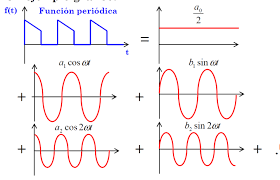
\includegraphics[scale=1.1]{periodica.png}
\end{figure}
\chapter{Rectificador}
Un rectificador es el dispositivo electrónico que permite convertir la corriente alterna en corriente continua. Esto se realiza utilizando diodos rectificadores, ya sean semiconductores de estado sólido, válvulas al vacío o válvulas gaseosas como las de vapor de mercurio (actualmente en desuso). Dependiendo de las características de la alimentación en corriente alterna que emplean, se les clasifica en monofásicos, cuando están alimentados por una fase de la red eléctrica, o trifásicos cuando se alimentan por tres fases.
Atendiendo al tipo de rectificación, pueden ser de media onda, cuando solo se utiliza uno de los semiciclos de la corriente, o de onda completa, donde ambos semiciclos son aprovechados. El tipo más básico de rectificador es el rectificador monofásico de media onda, constituido por un único diodo entre la fuente de alimentación alterna y la carga.
\begin{figure}[H]
\centering
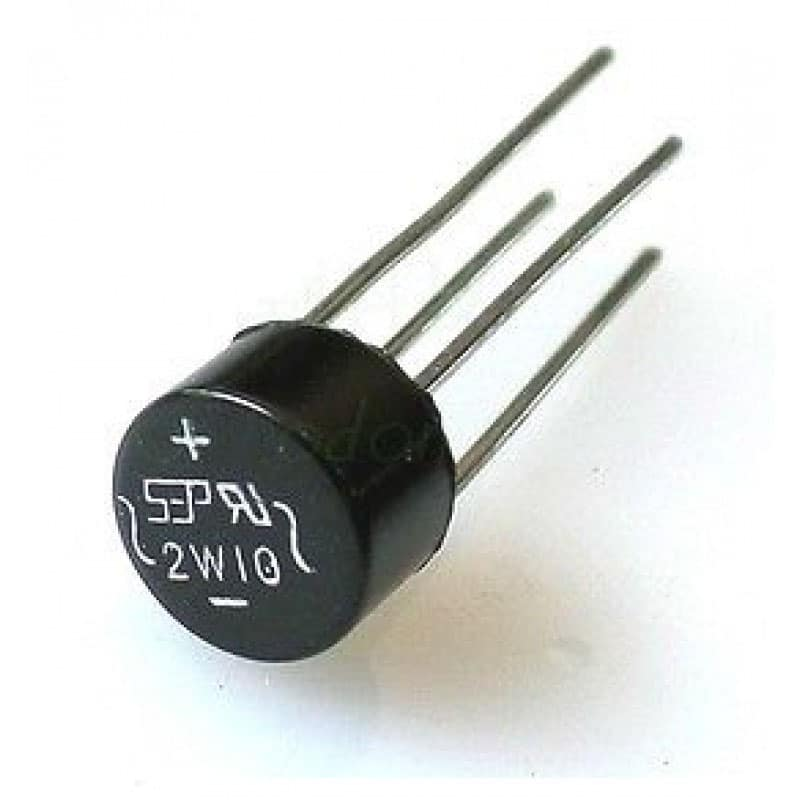
\includegraphics[scale=0.2]{rectificador.jpg}
\end{figure}
\begin{thebibliography}{99}  %%%este es un contador para el número de bibliografías utilizados.
\addcontentsline{toc}{chapter}{Bibliograf\'{\i}a} %%% Para introducir la bibliografía en el índice.
%\bibitem{Rahman}{Rahman,Aminur y Doe, Hidekazu; ``Ion transfer of tetraalkylammonium cations at an interface between 
%frozen aqueous solution and 1,2-dichloroethane".{\em{Journal of Electroanalytical Chemistry}} {\bfseries 424},159,(1997).}
\bibitem{Gro}{Boylestad, Robert M. ``Introducción al análisis de circuitos''. {\em{Pearson}}}
\bibitem{Gro}{Sadiku, Matthew N. ``Fundamemtos de circuitos eléctricos''. {\em{Mc Graw Hill}}}
%\bibitem{Ding}{Ding, Zhifeng. ``Spectroelectrochemistry and photoelectrochemistry of charge transfer at liquid/liquid
%interfaces". {\em {Tesis, EPFL,}}(1999).}
%\bibitem{AL}{Alonso, Jose M. \em{Técnicas de mecanizado 1}}
%\bibitem{AL}{Alonso, Jose M. ``Técnicas de mecanizado 1". {\em{Paraninfo}} {\bfseries España-Madrid}, 6-20, (2001).}
%\bibitem{Samec2}{Samec Z., Lhotsky A., Jänchenová H., y Marecek, V. ``Interfacial tension and impedance measurements
%of interfaces between two inmiscible electrolyte solutions". {\em{Journal of Electroanalytical Chemistry}} {\bfseries
%43}, 47, (2000).}
%\bibitem{Day}{Day R.A. y Underwood A.L. {\textit{Química Analítica Cuantitativa}},5ºed. Prentice-Hall, México, 1998. 45-48.}
%\bibitem{Keyser}{Farah Abud, Michel. ``Determinación de la vida útil en herramientales de corte endurecido por el proceso de borurización en pasta''. {\em{Instituto tecnológico y de estudios superiores de Monterrey}}}
%\bibitem{Zolotorevski}{Escalona, I. ``Máquinas: herramientas por arranque de viruta.''.{\em{El Cid Editor.}}}
%\bibitem{Lasheras}{Lasheras. ``Tecnología de los Materiales Industriales''.} 
%\bibitem{Dieter}{Dieter. ``Metalurgia mecánica''.}
%\bibitem{Apraiz}{Apraiz, J. ``Tratamiento Térmico de los Aceros''.}
%\bibitem{Smith}{Smith, William F. y Ph.D. Hashemi, Javad ``Ciencia e ingeniería de materiales". {\em{
%Madrid: McGraw-Hill, Interamericana de España.}} 570, (2004).} 
%\bibitem{Callister}{Callister, William D. y Rethwisch, David G. ``Introducción a la ingeniería de los materiales''. %{\em{Barcelona Reverté.}}, 960, (2007).} 
%\bibitem{Askeland}{Askeland, Donald R., Pradeep P. Phulé y Wright, Wendelin J. ``Ciencia e ingeniería de los materiales''.{\em{México, D.F. Internacional Thomson Editores.}} {\textit{$6^{ta}$ edición}}, 1004, (2012).}
%\bibitem{HARDBANDING}{Tabla de conversión de escala de durezas. \begin{verbatim}http://%hardbandingsolutions.com/postle_sp/hardness.php
%\end{verbatim}}
%\bibitem{HE}{Fresadora. \begin{verbatim} http://lizdenbow.blogspot.com/
%\end{verbatim}}
%\bibitem{ASTM}{Normas ASTM.}
%\bibitem{NTP}{Normas NTP.}
\end{thebibliography}
\end{document}
